\documentclass[11pt,letterpaper]{article}
\usepackage[lmargin=1in,rmargin=1in,bmargin=1in,tmargin=1in]{geometry}
\usepackage{style/quiz}
\usepackage{style/commands}

% -------------------
% Content
% -------------------
\begin{document}
\thispagestyle{title}


% Quiz 1
\quizsol \textit{True/False}: If $P$ is the proposition $6 < 5$ and $Q$ is the proposition, ``Earth is a planet,'' then the logical statement $P \to Q$ is false. \pspace

\sol The statement is \textit{false}. Recall that the truth table for $P \to Q$ is as follows: \par
	\begin{table}[!ht]
	\centering
	\begin{tabular}{c|c|c}
	$P$ & $Q$ & $P \to Q$ \\ \hline
	$T$ & $T$ & $T$ \\
	$T$ & $F$ & $F$ \\
	$F$ & $T$ & $T$ \\
	$F$ & $F$ & $T$
	\end{tabular}
	\end{table} \par
Here, $P$ is the proposition $P: 6 < 5$ and $Q$ is the proposition $Q$: ``Earth is a planet.'' It is clear that $P$ is false and $Q$ is true. But then examining the logic table above, we can see that $P \to Q$ is true. \pvspace{1.5cm}



% Quiz 2
\quizsol \textit{True/False}: $\neg (P \to \neg Q) \equiv P \wedge Q$ \pspace

\sol The statement is \textit{true}. To determine if two propositions are logically equivalent, one can either examine the truth table or apply logical rules to obtain one logical expression from the other. If we construct a truth table, we have\dots \par
	\begin{table}[!ht]
	\centering
	\begin{tabular}{c|c||c|c|c||c}
	$P$ & $Q$ & $\neg Q$ & $P \to \neg Q$ & $\neg (P \to \neg Q)$ & $P \wedge Q$ \\ \hline
	$T$ & $T$ & $F$ & $F$ & $T$ & $T$ \\
	$T$ & $F$ & $T$ & $T$ & $F$ & $F$ \\
	$F$ & $T$ & $F$ & $T$ & $F$ & $F$ \\
	$F$ & $F$ & $T$ & $T$ & $F$ & $F$
	\end{tabular}
	\end{table}
Because for each possible pair of choices for $P$ and $Q$ the outputs for $\neg (P \to \neg Q)$ and $P \wedge Q$ match, $\neg (P \to \neg Q) \equiv P \wedge Q$. Alternatively, we can transform one into the other by applying logical equivalences (recall $P \to Q \equiv \neg P \vee Q$ or $\neg (P \to Q) \equiv P \wedge \neg Q$):
	\[
	\neg (P \to \neg Q) \equiv \neg (\neg P \vee \neg Q) \equiv \neg (\neg P) \wedge \neg (\neg Q) \equiv P \wedge Q.
	\]  \pvspace{0.5cm}



% Quiz 3
\quizsol \textit{True/False}: The logic corresponding to the circuit shown below is the proposition:
	\[
	(\neg P \wedge Q) \vee \neg Q.
	\]
	\begin{figure}[!ht]
	\centering
	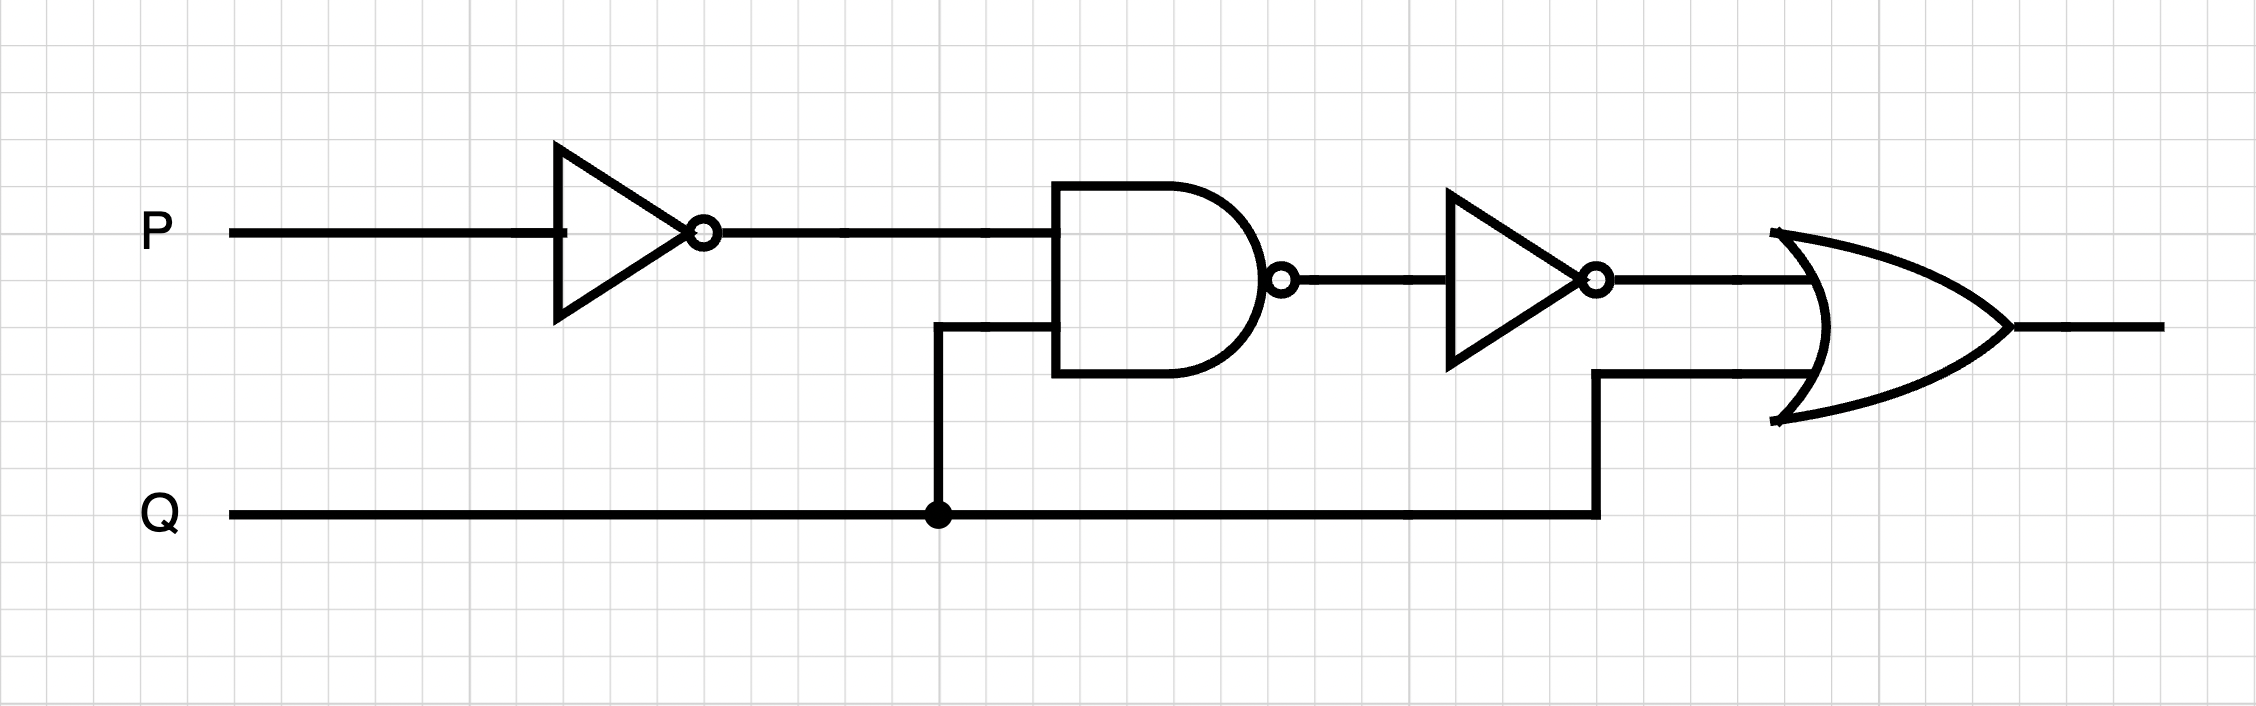
\includegraphics[width=0.74\textwidth]{images/circuit}
	\end{figure} \par

\newpage

\sol The statement is \textit{false}. We can trace through the circuit. We see that the current from $P$ passes through a NOT gate and we obtain $\neg P$. This then feeds into an AND gate along with $Q$ so that we obtain $\neg P \wedge Q$. The resulting current is then passed through a NOT gate, obtaining $\neg (\neg P \wedge Q)$. This finally reaches an OR gate---along with $Q$---to obtain $\neg (\neg P \wedge Q) \vee Q$. We can see a diagrammatic explanation below. \par
	\begin{figure}[!ht]
	\centering
	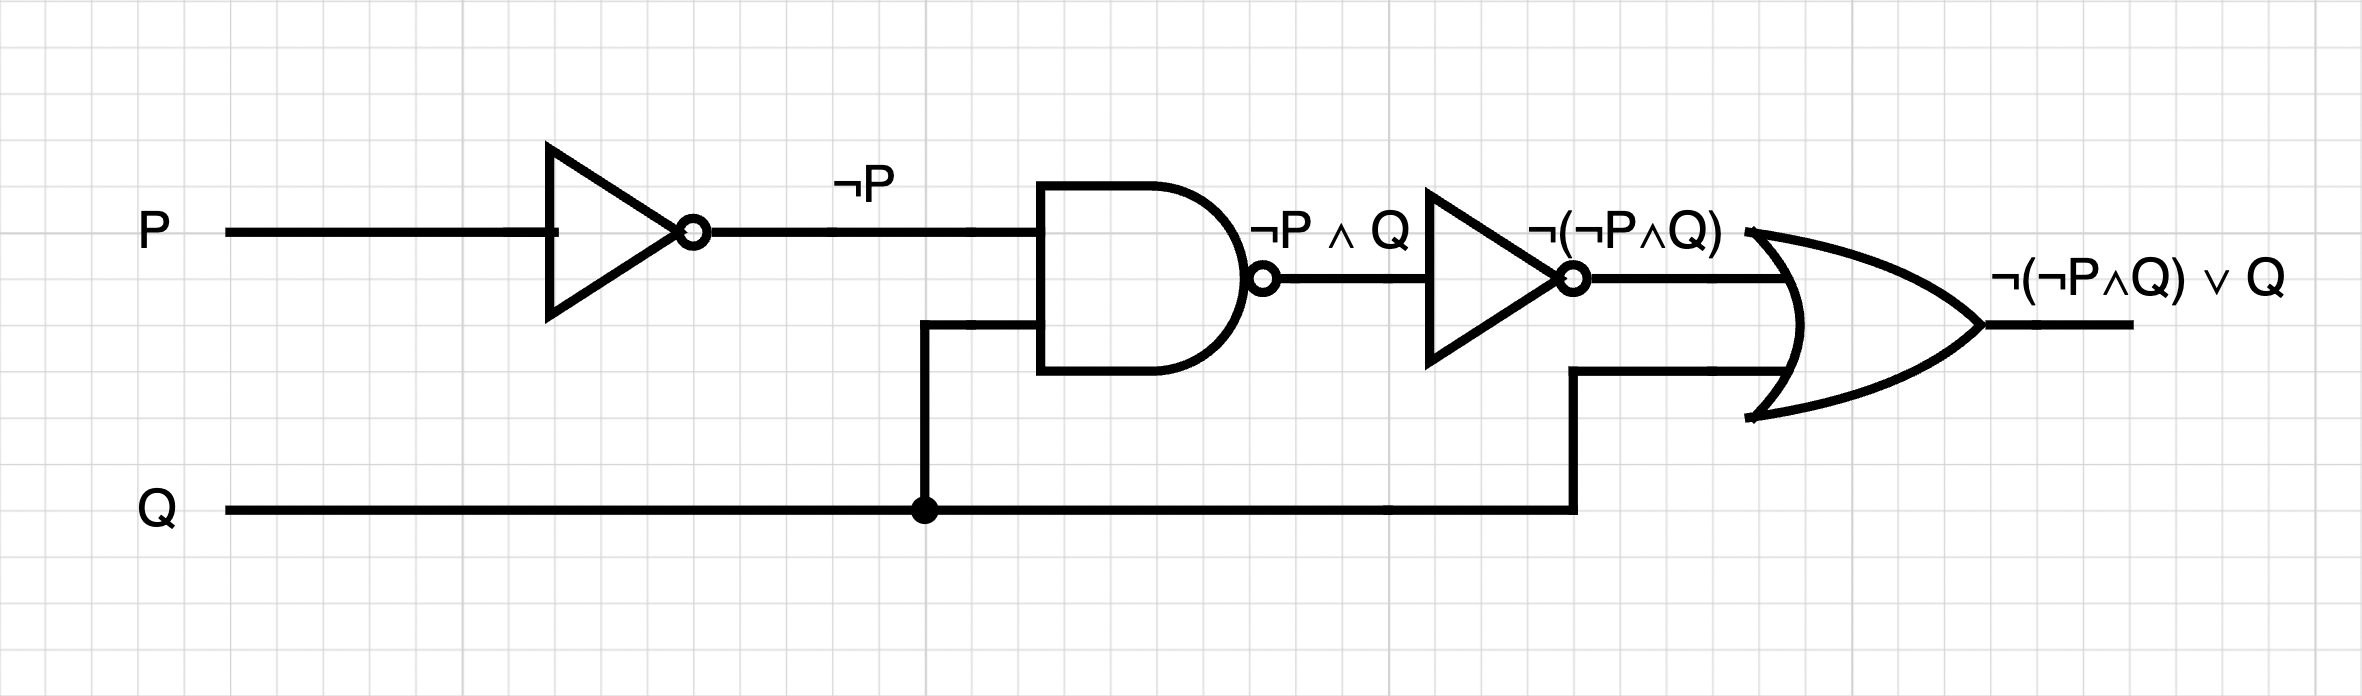
\includegraphics[width=0.74\textwidth]{images/circuit_sol}
	\end{figure} \pvspace{1.5cm}



% Quiz 4
\quizsol \textit{True/False}: Let the universe $\mathcal{U}$ be the set of real numbers and define $P(x)$ to be the predicate $P(x): x^2 + x - 4 \geq 0$. Then $(\forall x) \big(\neg P(x) \big)$ is true. \pspace

\sol The statement is \textit{false}. If $P(x): x^2 + x - 4 \geq 0$, then $\neg P(x): x^2 + x - 4 < 0$. But then $(\forall x) \big(\neg P(x) \big)$ is the statement, ``For all $x$, $x^2 + x - 4 < 0$.'' Now if $x= 1$, we have $\neg P(1) \colon 1^2 + 1 - 4 < 0$, i.e. $-2 < 0$, which is true. If $x= 0$, we have $\neg P(0) \colon 0^2 + 0 - 4 < 0$, i.e. $-4 < 0$, which is true. However, while $(\forall x) \big(\neg P(x) \big)$ is clearly true for \textit{some} (we found at least two), it is not true \textit{for all} $x$. As a counterexample, let $x= 10$. Then $\neg P(10) \colon 10^2 + 10 - 4 < 0$, which is $104 < 0$---clearly false. Therefore, $\neg P(x)$ is not true for all $x$. But then $(\forall x) \big(\neg P(x) \big)$ is false. \pvspace{1.5cm}




% Quiz 5
\quizsol \textit{True/False}: Let the domain of $x, y$ be the integers. Then $(\exists! x)(\forall y)(x + 2y= 5)$. \pspace

\sol The statement is \textit{false}. The logical proposition $(\exists! x)(\forall y)(x + 2y= 5)$ in words states, ``There exists a unique $x$ such that for all $y$, $x + 2y= 5$.'' Suppose that there were such a $x$, say $x_0$. Then we know that $x_0 + 2y= 5$ for all $y$. In particular, $x_0$ satisfies this equality when $y= 0$. But then we know that $x_0= 5$. But also, it must satisfy the equality when $x= 1$. But then $x_0 + 2= 5$ so that $x_0$. Then there is not a unique $x$ that works for all $y$! Therefore, the statement is false. Note that if we reverse the quantifiers, the statement is true: $(\forall y)(\exists! x)(x + 2y= 5)$. In this case, this is the statement, ``For all $y$, there exists a unique $x$ such that $x + 2y= 5$.'' If you were given any $y$, define $x_0:= 5 - 2y$. But then $x + 2y= (5 - 2y) + 2y= 5$. So there exists such an $x$. Is it unique? Well if there were two or more $x$ values that worked for some $y$, say two of them are $x_0$ and $\tilde{x}_0$, then we have $x_0 + 2y= 5= \tilde{x}_0 + 2y$. But then $x_0 + 2y= \tilde{x}_0 + 2y$. Subtracting $2y$, we have $x_0 = \tilde{x}_0$. Therefore, there can only be one such $x$. Because we have found one, we know that the statement that for all $y$, there exists a unique $y$ such that $x + 2y= 5$ is true. 





\newpage





% Quiz 6
\quizsol \textit{True/False}:  $\{ 1, 2 \} \subseteq \{ \varnothing, \{ 1 \}, \{ 2 \}, \{ 1, 2 \} \}$ \pspace

\sol The statement is \textit{false}. We know that $A \subseteq B$ if and only if for all $a \in A$, we have $a \in B$. We test every element of the set $\{ 1, 2 \}$. The first element is 1. However, $1 \notin \{ \varnothing, \{ 1 \}, \{ 2 \}, \{ 1, 2 \} \}$. [Note that $1 \notin \{ \varnothing, \{ 1 \}, \{ 2 \}, \{ 1, 2 \} \}$ but $\{ 1 \} \in \{ \varnothing, \{ 1 \}, \{ 2 \}, \{ 1, 2 \} \}$.] However, we do have $\{ 1, 2 \} \notin \{ \varnothing, \{ 1 \}, \{ 2 \}, \{ 1, 2 \} \}$. \pvspace{1.5cm}



% Quiz 7
\quizsol \textit{True/False}: $\displaystyle\bigcap_{n \in \mathbb{N}} \left( -\frac{1}{n}, \frac{1}{n} \right)= \varnothing$ \pspace

\sol The statement is \textit{false}. For $n= 1$, the set $(-\frac{1}{n}, \frac{1}{n})$ is the interval $(-1, 1)$. For $n= 2$, the set $(-\frac{1}{n}, \frac{1}{n})$ is the interval $(-\frac{1}{2}, \frac{1}{2})$. For $n= 3$, the set $(-\frac{1}{n}, \frac{1}{n})$ is the interval $(-\frac{1}{3}, \frac{1}{3})$. Note that $0$ is an element of all these sets. Generally, we have $0 \in (-\frac{1}{n}, \frac{1}{n})$ for all $n \in \mathbb{N}$. But then we know that $0 \in \displaystyle\bigcap_{n \in \mathbb{N}} \left( -\frac{1}{n}, \frac{1}{n} \right)$. This is sufficient to demonstrate that this is not empty. [Note that it is actually true that $\displaystyle\bigcap_{n \in \mathbb{N}} \left( -\frac{1}{n}, \frac{1}{n} \right)= \{ 0 \}$---though this takes more work to prove.] \pvspace{1.5cm}



% Quiz 8
\quizsol \textit{True/False}: Let $E(n)$ denote the relation from $\mathbb{N}$ to $\mathbb{Z}^{\geq 0}$ given by the rule that $E(n)$ is the number of positive even integers less than or equal to $n$. Then this relation is a function with $E(5)= 2$, i.e. 2 is in the image of 5, and 10 in the preimage of 5. \pspace

\sol The statement is \textit{true}. There are several claims here. First, the claim that $E(n): \mathbb{N} \to \mathbb{Z}^{\geq 0}$ is a function. Given some $n \in \mathbb{N}$, there is a single number of positive even integers $\leq n$. But then for every input for $E(n)$, there is only one possible output. Therefore, $E(n)$ is a function from $\mathbb{N}$ to $\mathbb{Z}^{\geq 0}$. For 2 to be in the image of 5, we need $E(5)= 2$. There are two positive even integers $\leq 5$ (namely, 2 and 4) so that 2 is in the image of 5. For 10 to be in the preimage of 5, we would have to have $E(10)= 5$. Note that there are 5 positive even integers $\leq 10$ (namely 2, 4, 6, 8, 10). Therefore, 10 is in the preimage of 5. \pvspace{1.5cm}



% Quiz 9
\quizsol \textit{True/False}: Let $f: X \to Y$ be a function. Then $f^{-1}$ will be a function if and only if the preimage set satisfies the following: $(\forall y \in \text{im } f)(\exists x \in X)(f^{-1}(y)= x)$. \pspace

\sol The statement is \textit{false}. Take for example the function $f: \mathbb{R} \to \mathbb{R}^{\geq 0}$ given by $f(x)= x^2$. For all $y \in \mathbb{R}^{\geq 0}$, there exists an $x \in \mathbb{R}$ such that $f(x)= y$, namely $\pm\sqrt{y}$. But if $y > 0$, then there are two possibilities: $+\sqrt{y}$ and $-\sqrt{y}$. But this function $f(x)$ has $f^{-1}$ with the property that $(\forall y \in \text{im }f)(\exists x \in X)(f^{-1}(y)= x)$. If we want $f^{-1}$ to be a function, we require $(\forall y \in \text{im }f)(\exists! x \in X)(f^{-1}(y)= x)$. 





\newpage




% Quiz 10
\quizsol \textit{True/False}: Suppose that $f: A \to B$ and $g: B \to C$ are functions and that $g \circ f$ is injective. Then it must be that $f$ is injective. \pspace

\sol The statement is \textit{true}. Observe that $g \circ f: A \to C$. Suppose $f$ were not injective. Then there are two values in $A$, say $a_1, a_2$, such that $a_1 \neq a_2$ and $f(a_1)= f(a_2)$. But then we have\dots
	\[
	\begin{aligned}
	f(a_1)&= f(a_2) \\
	g(f(a_1))&= g(f(a_2)) \\
	(g \circ f)(a_1)&= (g \circ f)(a_2)
	\end{aligned}
	\] 
But then there are two values in the domain of $g \circ f$, namely $a_1, a_2$ such that $a_1 \neq a_2$ but $(g \circ f)(a_1)= (g \circ f)(a_2)$. But then $g \circ f$ is not injective, contrary to what we were told. Our assumption that $f$ was not injective must then be wrong. Therefore, it must be that $f$ is injective. \pvspace{1.5cm}



% Quiz 11
\quizsol \textit{True/False}: Fix an integer $n > 1$ and let $\{ a_n \}_{n \in \mathbb{N}}$ and $\{ b_n \}_{n \in \mathbb{N}}$ be sequences. Then $\displaystyle \prod_{k=1}^n a_n b_n= \prod_{k=1}^n a_n \cdot \prod_{k=1}^n b_n$ but $\displaystyle \sum_{k=1}^n a_n b_n \neq \sum_{k=1}^n a_n \cdot \sum_{k=1}^n b_n$. \pspace

\sol The statement is \textit{true}. It is true that $\displaystyle \prod_{k=1}^n a_n b_n= \prod_{k=1}^n a_n \cdot \prod_{k=1}^n b_n$. For instance, if $n=2$, we have\dots
	\[
	\prod_{k=1}^2 a_n b_n= a_1 b_1 \cdot a_2 b_2= (a_1 a_2) \cdot (b_1 b_2)= \prod_{k=1}^2 a_n \cdot \prod_{k=1}^2 b_n
	\]
We can always rearrange the terms in this way for any $n$. Therefore, the statement is true for products. \pspace

However, even in the case of $n= 2$, the statement is untrue for sums. For example, if $n= 2$ in $\displaystyle \sum_{k=1}^n a_n b_n \neq \sum_{k=1}^n a_n \cdot \sum_{k=1}^n b_n$, then we have\dots
	\[
	\begin{aligned}
	\sum_{k=1}^2 a_n b_n&= a_1b_1 + a_2b_2 \\[0.3cm]
	\sum_{k=1}^2 a_n \cdot \sum_{k=1}^n b_2&= (a_1 + a_2) \cdot (b_1 + b_2)= a_1b_1 + a_1b_2 + a_2b_1 + a_2 b_2
	\end{aligned}
	\]
While this may be true for some sequences $\{ a_n \}_{n \in \mathbb{N}}$ and $\{ b_n \}_{n \in \mathbb{N}}$, it will not generally be true. The `issues' the distributive property cause for larger $n$ make this even `more untrue.' 





\newpage





% Quiz 12
\quizsol \textit{True/False}: Suppose that $a_{n+2}= 6a_n - a_{n+1}$ with $a_0= 4$ and $a_1= 3$. Then the characteristic polynomial is given by the equation $x^2= 6 - x$, i.e. the characteristic polynomial is $x^2 + x - 6$. Because $x^2 + x - 6= (x + 3)(x - 2)$ has roots $-3, 2$, the general solution is $a_n= c_1(-3)^n + c_2 2^n$. The specific solution is then $a_n= (-3)^n + 3 \cdot 2^n$. \pspace

\sol The statement is \textit{true}. Because $a_{n+2}= 6a_n - a_{n+1}$ and the `lowest' term involved is $n$, we give the $n$th term power 0 for $x$. Then we have $x^{0 + 2}= 6 x^0 - x^{0 + 1}$. This is $x^2= 6 - x$. We then have $x^2 + x - 6= 0$. Therefore, the characteristic polynomial for this homogeneous linear recurrence relation is $x^2 + x - 6$. This polynomial has roots $-3$ and 2 because $x^2 + x - 6= 0$ is equivalent to $(x + 3)(x - 2)= 0$, which has solutions $x= -3$ and $x= 2$. Therefore, we know that $a_n= c_1 (-3)^n + c_2 \cdot 2^n$. Now we use the fact that when $n= 0$, we have $a_0= 4$, and when $n= 1$, we have $a_1= 3$. But then we have\dots
	\[
	\begin{aligned}
	4&= a_0= c_1 (-3)^0 + c_2 \cdot 2^0= c_1 + c_2 \\[0.3cm]
	3&= a_1= c_1 (-3)^1 + c_2 \cdot 2^1= -3c_1 + 2c_2
	\end{aligned}
	\]
This is a linear system of two equations in two unknowns. Solving this system yields $c_1= 1$ and $c_2= 3$. Therefore, we have $a_n= (-3)^n + 3 \cdot 2^n$. \pvspace{1.5cm}



% Quiz 13
\quizsol \textit{True/False}: $6^{2022} \equiv 1 \mmod 5$ \pspace

\sol The statement is \textit{true}. Using the division algorithm, we know that $6= 1(5) + 1$. But then we know that $6 \equiv 1 \mmod 5$. But then we have\dots
	\[
	6^{2022} \equiv 1^{2022} \equiv 1 \mmod 5
	\] \pvspace{1.5cm}



% Quiz 14
\quizsol \textit{True/False}: There is a unique solution to the following system of linear congruences:
	\[
	\begin{aligned}
	2x - 1 &\equiv 2 \mmod 3 \\
	x &\equiv 0 \mmod 5 \\
	6x &\equiv 5 \mmod 7
	\end{aligned}
	\] 

\sol The statement is \textit{true}. The first congruence is $2x - 1 \equiv 2 \mmod 3$. Adding 1 to both sides, we see that this is equivalent to $2x \equiv 3 \equiv 0 \mmod 3$. Because $\gcd(2, 3)= 1$, we know that $2^{-1}$ exists mod 3. In fact, because $2 \cdot 2 \equiv 4 \equiv 1 \mmod 3$. Therefore, $2^{-1} \equiv 2 \mmod 3$. Therefore, $2x \equiv 0 \mmod 3$ implies $2^{-1} \cdot 2x \equiv 2^{-1} \cdot 0 \mmod 3$. This is $x \equiv 0 \mmod 3$. In the last congruence, because $\gcd(6, 7)= 1$, we know that $6^{-1}$ exists mod 7. In fact, because $6 \cdot 6 \equiv 36 \equiv 1 \mmod 7$, we know that $6^{-1} \equiv 6 \mmod 7$. But then $6x \equiv 5 \mmod 7$ implies $6^{-1} \cdot 6x \equiv 6^{-1} \cdot 5 \mmod 7$. But this is $x \equiv 6 \cdot 5 \equiv 30 \equiv 2 \mmod 7$. The original system of congruences is then equivalent to\dots
	\[
	\begin{aligned}
	x &\equiv 0 \mmod 3 \\
	x &\equiv 0 \mmod 5 \\
	x &\equiv 2 \mmod 7
	\end{aligned}
	\] 
This system now has the `proper form' to apply the Chinese Remainder Theorem. Because $\gcd(3, 5, 7)= 1$, we know there exists a unique solution to the system of congruences. In fact, we have solution\dots
	\[
	x= \sum a_i N_i M_i= 0 \cdot 2 \cdot 35 + 0 \cdot 1 \cdot 21 + 2 \cdot 1 \cdot 15= 0 + 0 + 30= 30 
	\]
The solution is then the congruence class of 30 modulo $3 \cdot 5 \cdot 7= 105$. Therefore, the solution is 30, i.e. $[30]= \{ \ldots, -720, -570, -420, -270, -120, 30, 180, 330, 480, 630, 780, \ldots \}$. \pvspace{1.5cm}



% Quiz 15
\quizsol \textit{True/False}: The number $1$ is prime. \pspace

\sol The statement is \textit{false}. A prime number is an integer greater than 1 which has no proper divisors. Because 1 is not greater than 1, 1 cannot be prime. Note that 1 is also not composite. To be composite, an integer need have proper divisors. However, the only divisor of 1 is 1. Therefore, 1 also cannot be composite. This shows 1 is neither prime nor composite. \pvspace{1.5cm}



% Quiz 16
\quizsol \textit{True/False}: Using the division algorithm to divide $-10$ by $3$, we have $-10= 3(3) + 1$. \pspace

\sol The statement is \textit{false}. Recall that given $a, b \in \mathbb{Z}$ with $a \neq 0$, we can write $b= qa + r$ for some $q, r \in \mathbb{Z}$ and $0 \leq r < a$. Clearly, the statement is false because $3(3) + 1= 9 + 1= 10 \neq -10$. The multiple of 3 that is less than or equal to $-10$ is $-12$. Because $-10= -12 + 2$, we have $-10= -4(3) + 2$. Because $-4, 2 \in \mathbb{Z}$ and $0 \leq 2 < 3$, we have expressed $-10$ divided by 3 using the division algorithm. Note that one cannot use $-10= -3(3) - 1$ because it is not the case that $0 \leq -1 < 3$. \pvspace{1.5cm}



% Quiz 17
\quizsol \textit{True/False}: The number $2B002B$ in base-10 is 2818091. \pspace 

\sol The statement is \textit{true}. The number 2B002B is in hexadecimal. Converting this to base-10 (and recalling $A= 10$, $B= 11$, $C= 12$, $D= 13$, $E= 14$, and $F= 15$), we have\dots
	\[
	2B002B= 2 \cdot 16^5 + 11 \cdot 16^4 + 0 \cdot 16^3 + 0 \cdot 16^2 + 2 \cdot 16^1 + 11 \cdot 16^0= 2097152 + 720896 + 0 + 0 + 32 + 11= 2818091
	\]



%% Quiz 18
%\quizsol \textit{True/False}: If $A, B$ are $n \times n$ matrices, then $AB= BA$. \pspace


% If $n$ is sufficiently large, then the number of dearrangements of $n$ is approximately $n!/e$.


% 20
% The number of ways of choosing a committee of 10 people with a president and vice president from 120 people is $_{120}C_{10} \cdot \phantom{}_{10}C_2$. 




\end{document}